\documentclass[11pt, a4paper]{article}

% === PACKAGES ===
\usepackage{arxiv}
\usepackage[utf8]{inputenc}
\usepackage[T1]{fontenc}
\usepackage{url}
\usepackage{booktabs}
\usepackage{amsfonts}
\usepackage{nicefrac}
\usepackage{microtype}
\usepackage{graphicx}
\usepackage{amsmath, amssymb, amsthm}
\usepackage{natbib}
\usepackage{doi}
\usepackage{hyperref}
\usepackage{listings}
\usepackage{float}
\usepackage{xcolor}
\usepackage{fancyhdr}
\usepackage{subcaption}
\usepackage[nomarkers,notables]{endfloat}

\lstset{
  language=Python,
  basicstyle=\ttfamily\small,
  keywordstyle=\color{blue!70!black},
  commentstyle=\color{gray!70!black},
  stringstyle=\color{orange!80!black},
  showstringspaces=false,
  frame=single,
  numbers=left,
  numberstyle=\tiny,
  numbersep=6pt,
  columns=fullflexible,
  breaklines=true,
  extendedchars=true,
  inputencoding=utf8,
  literate={α}{{\(\alpha\)}}1
           {β}{{\(\beta\)}}1
           {γ}{{\(\gamma\)}}1
           {δ}{{\(\delta\)}}1
           {ε}{{\(\epsilon\)}}1
           {λ}{{\(\lambda\)}}1
           {μ}{{\(\mu\)}}1
           {π}{{\(\pi\)}}1
           {σ}{{\(\sigma\)}}1
           {τ}{{\(\tau\)}}1
           {φ}{{\(\phi\)}}1
           {ψ}{{\(\psi\)}}1
           {∈}{{\(\in\)}}1
           {∑}{{\(\sum\)}}1
           {Σ}{{\(\Sigma\)}}1
           {∏}{{\(\prod\)}}1
           {√}{{\(\sqrt\)}}1
           {ℓ}{{\(\ell\)}}1
           {η}{{\(\eta\)}}1
}

% === MACROS ===
\newtheorem{theorem}{Theorem}
\newtheorem{proposition}{Proposition}
\newtheorem{lemma}{Lemma}
\newtheorem{definition}{Definition}
\theoremstyle{remark}
\newtheorem{remark}{Remark}
\newcommand{\R}{\mathbb{R}}
\newcommand{\E}{\mathbb{E}}

% === RUNNING HEADERS ===
\renewcommand{\shorttitle}{Day-Ahead Electricity Prices FR-DE}
\fancypagestyle{main}{%
  \fancyhf{}
  \fancyhead[L]{\shorttitle}
  \fancyhead[R]{\scshape Statistical Report}
  \fancyfoot[C]{\thepage}
  \renewcommand{\headrulewidth}{0.4pt}
  \renewcommand{\footrulewidth}{0pt}
}

% === METADATA ===
\title{Dependence, Extremes, and Temporal Clustering in\\
French and German Day-Ahead Electricity Prices in 2025}

\author{
    Lucas Jung \\
    Graduate Student in Artificial Intelligence \\
    École Polytechnique \\
    Palaiseau, France \\
    \texttt{lucas.jung@polytechnique.org} \\
    \And
    Thaïs Roussel \\
    Graduate Student in Applied Mathematics \\
    École Polytechnique \\
    Palaiseau, France \\
    \texttt{thais.roussel@polytechnique.edu} \\
    \And
    Maxime Puech \\
    Graduate Student in Applied Mathematics \\
    École Polytechnique \\
    Palaiseau, France \\
    \texttt{maxime.puech@polytechnique.edu} \\
}

\begin{document}
\maketitle
\pagestyle{main}

\begin{abstract}
This report studies hourly day-ahead electricity prices in France and Germany over the year 2025 using data from the ENTSO-E Transparency Platform. Our objective is to understand how market tensions appear, how they persist over time, and how they propagate across the two markets. To do so, we build a unified statistical analysis around a single dataset and a single research question: when the market becomes stressed, do French and German prices become more dependent, and do extreme episodes cluster in time?

We first clean and synchronize the hourly series, then study their temporal structure through standard linear time-series tools. We next analyze extreme price events using methods from extreme value theory in order to characterize rare positive spikes and negative prices, and to define meaningful thresholds for subsequent event-based modeling. We then investigate the cross-market dependence structure using copulas, comparing Gaussian, Gumbel, and Clayton specifications in both calm and stressed regimes. Finally, we model the temporal clustering of extreme events through univariate and bivariate Hawkes processes, which allow us to distinguish exogenous shocks from endogenous excitation and to quantify cross-market propagation.

Our results highlight three main features of the French-German day-ahead market in 2025: a strong common temporal structure, a dependence pattern that becomes especially relevant in the tails, and a clear clustering of extreme events over time. Together, these findings show that the interaction between the two markets cannot be reduced to simple linear correlation alone, but involves asymmetric tail dependence and self-exciting dynamics that are important for understanding stress episodes in the European electricity system.
\end{abstract}

% ==========================================
% 1. INTRODUCTION
% ==========================================
\section{Introduction}
\label{sec:intro}
Electricity prices provide a natural setting for statistical analysis because they combine strong temporal regularities, abrupt stress episodes, and cross-market dependence. In European day-ahead markets, prices are determined on an hourly basis for the following day, which yields a regular time series that is well suited to linear time-series tools while also exhibiting extreme events such as very high prices or negative prices.

In this report, we focus on the French and German day-ahead electricity markets over the year 2025. Our goal is not to apply several disconnected methods to the same dataset, but rather to answer a single question: when market conditions become stressed, do the French and German price series become more dependent, and do extreme events propagate over time and across markets?

To address this question, we use a common cleaned dataset extracted from the ENTSO-E Transparency Platform and organize the analysis in four steps. We first study the marginal temporal structure of the hourly series using linear time-series methods. We then analyze the tails of the distribution using extreme-value tools. Next, we investigate cross-market dependence through copulas. Finally, we model the temporal clustering of extreme events with Hawkes processes. This progression reflects the logic of the course: margins before dependence, thresholds motivated by extreme-value analysis, and point-process modeling for temporal clustering that copulas alone cannot capture.


% ==========================================
% 2. DATA AND PREPROCESSING
% ==========================================
\section{Data and Preprocessing}
\label{sec:data}
The data used in this report come from the ENTSO-E Transparency Platform, under item \texttt{EnergyPrices\_12.1.D\_r3}. This dataset provides day-ahead electricity prices for each bidding zone and each market time unit, in currency per MWh. We downloaded the 12 monthly files corresponding to the year 2025 and concatenated them into a single panel dataset.

We then filtered the data to retain only the French and German bidding zones and restricted attention to hourly day-ahead observations. Timestamps were recorded in UTC and were carefully standardized before analysis. After merging the monthly files and removing possible duplicates by market zone and timestamp, we obtained two synchronized hourly series covering the full year 2025.

The final cleaned dataset serves as the common empirical basis for all parts of the report. This is important because the time-series, extreme-value, copula, and Hawkes analyses should not be viewed as separate projects, but as complementary perspectives on the same underlying market dynamics.


% ==========================================
% 3. LINEAR TIME SERIES
% ==========================================
\section{Linear Time-Series Analysis}
\label{sec:timeseries}
\documentclass[11pt, a4paper]{article}

% === PACKAGES ===
\usepackage{booktabs}
\usepackage{amsfonts}
\usepackage{nicefrac}
\usepackage{microtype}
\usepackage{graphicx}
\usepackage{amsmath, amssymb, amsthm}
\usepackage{natbib}
\usepackage{doi}
\usepackage{hyperref}
\usepackage{listings}
\usepackage{float}
\usepackage{xcolor}
\usepackage{fancyhdr}
\usepackage{subcaption}
\usepackage[nomarkers,notables]{endfloat}

\lstset{
  language=Python,
  basicstyle=\ttfamily\small,
  keywordstyle=\color{blue!70!black},
  commentstyle=\color{gray!70!black},
  stringstyle=\color{orange!80!black},
  showstringspaces=false,
  frame=single,
  numbers=left,
  numberstyle=\tiny,
  numbersep=6pt,
  columns=fullflexible,
  breaklines=true,
  extendedchars=true,
  inputencoding=utf8,
  literate={α}{{\(\alpha\)}}1
           {β}{{\(\beta\)}}1
           {γ}{{\(\gamma\)}}1
           {δ}{{\(\delta\)}}1
           {ε}{{\(\epsilon\)}}1
           {λ}{{\(\lambda\)}}1
           {μ}{{\(\mu\)}}1
           {π}{{\(\pi\)}}1
           {σ}{{\(\sigma\)}}1
           {τ}{{\(\tau\)}}1
           {φ}{{\(\phi\)}}1
           {ψ}{{\(\psi\)}}1
           {∈}{{\(\in\)}}1
           {∑}{{\(\sum\)}}1
           {Σ}{{\(\Sigma\)}}1
           {∏}{{\(\prod\)}}1
           {√}{{\(\sqrt\)}}1
           {ℓ}{{\(\ell\)}}1
           {η}{{\(\eta\)}}1
}

% === MACROS ===
\newtheorem{theorem}{Theorem}
\newtheorem{proposition}{Proposition}
\newtheorem{lemma}{Lemma}
\newtheorem{definition}{Definition}
\theoremstyle{remark}
\newtheorem{remark}{Remark}
\newcommand{\R}{\mathbb{R}}
\newcommand{\E}{\mathbb{E}}

% === CUSTOM FORMULAS ===

\newcommand{\T}{\mathcal{T}}
\newcommand{\Cov}{\mathrm{Cov}}
\newcommand{\ARMA}{\mathrm{ARMA}}
\newcommand{\ARIMA}{\mathrm{ARIMA}}
\newcommand{\AR}{\mathrm{AR}}
\newcommand{\GARCH}{\mathrm{GARCH}}
\newcommand{\ARCH}{\mathrm{ARCH}}
\newcommand{\entFF}[2]{[\![ #1, #2 ]\!]}
\newcommand{\N}{\mathbb{N}}
\newcommand{\code}[1]{\texttt{#1}}
\newcommand{\Z}{\mathbb{Z}}

\begin{document}

\subsection{Framework}

In order to discuss the dynamics of the data based on time-series analysis, let us first explain some notations. Whether it is for french or german energy prices, we'll consider the time space:
\begin{align*}
\T = \{ \mathrm{hour}\!:\!\mathrm{min} \mid \mathrm{hour} \in \entFF{0}{23}, \; \mathrm{min} \in \{0, 15, 30, 45\}\}.
\end{align*}
Every process $X$ considered in this section will take as events the times in the space $\T$, and will span from day $1$ to day $365$, meaning we'll write $(X_t)_t$ instead of $(X_t)_{t \in \entFF{1}{365}}$. Moreover, expectancies will be taken as if the times were chosen uniformly at random in $\T$.

\subsection{Test of stationarity}

\subsubsection{Expectancy function}

In order to modelise our data as $\ARMA(p,q)$ processes, we first need to assess if we can assume the data to be stationary. Let's recall that a process $(X_t)_t$ is said to be (weakly-)stationary if it's square-integrable, its expectancy function is constant and for all $0 \leq s \leq t$, $\Cov(X_s, X_t)$ only depends on $t-s$. To test the last two hypothesis, we need to run the computation of the expectancies and the autocovariance function.

\begin{table}[H]
\centering
\caption{Means and standard deviation of the mean prices per day.}
\label{tab:statio}
\begin{tabular}{lcc}
\toprule
Country & Mean price (€) & Ratio std/mean \\
\midrule
France & 61.08 & 0.32  \\
Germany-Luxembourg  & 89.39 & 0.31 \\
\bottomrule
\end{tabular}
\end{table}
The ratio between standard deviation and the mean helps on showing if the function $t \mapsto \E(X_t)$ is constant or not. Here, the ratio might seem too high. To try to circumvent this issue, we introduce the differentiation operator
\begin{align*}
\nabla \colon X \mapsto (X_t - X_{t-1})_t.
\end{align*}
By applying this operator $d \in \N^*$ times to a process $X$, it removes polynomial tendencies of degree $d-1$. Then, for example the process $\nabla^2 X$ could prove to have its expectancy function constant, and we could then try to modelise it as an $\ARMA$ process. To retrieve the initial process, one may note that:
\[ Y_t = Y_0 + \sum_{i=1}^t (\nabla Y)_t.\]

Figure \ref{fig:ratio_fr} shows the ratio between standard deviation and mean on the function $t \mapsto \E((\nabla^dX)_t)$ for $d$ varying from $0$ to $100$, while figure \ref{fig:ratio_de} shows the same for Germany. One may notice that the two best ratios are obtained for $d=0$ and $d=1$, meaning we'll be modelising one of the two as an $\ARMA$ process. The next step is to compute the autocovariance function.

\begin{figure}[H]
    \centering
    
\includegraphics[width=0.58\textwidth]{ratio_fr.png}
    \caption{Ratio std/mean of the expectancy function for the french prices process differentiated $n$ times.}
    \label{fig:ratio_fr}
\end{figure}

\begin{figure}[H]
    \centering
    
\includegraphics[width=0.58\textwidth]{ratio_de.png}
    \caption{Ratio std/mean of the expectancy function for the german prices process differentiated $n$ times.}
    \label{fig:ratio_de}
\end{figure}

\subsubsection{Autocovariance function}

For a stationary process, computing the autocovariance function is fairly easy. One only needs to compute:

\[ \gamma(n) = \Cov(X_n, X_0), \quad \text{ for every } n \in \N.\]
However, to test the stationarity, we'll be computing for every $n \in \N$,
\[ t \mapsto \Cov(X_{t+n}, X_t),\]
to test whether it is constant or not. We did this computation, and checked the mean and the standard deviation, to figure out which trajectory would be best. Figure \ref{fig:cov_fr} shows the ratio between standard deviation and mean for the autocovariance function, while figure \ref{fig:cov_de} shows the same for Germany. The trajectories depend on the number of times the process has been differentiated. It clearly shows that the best candidate to be modelised as an $\ARMA$ is the energy prices process itself.

\begin{figure}[H]
    \centering
    
\includegraphics[width=0.58\textwidth]{cov_fr.png}
    \caption{Ratio std/mean of the autocovariance function for the french prices process, with trajectories depending on the number of differentiations.}
    \label{fig:cov_fr}
\end{figure}

\begin{figure}[H]
    \centering
    
\includegraphics[width=0.58\textwidth]{cov_de.png}
    \caption{Ratio std/mean of the autocovariance function for the german prices process, with trajectories depending on the number of differentiations.}
    \label{fig:cov_de}
\end{figure}

\subsection{ARMA modelisation}

\subsubsection{With statsmodels}

The module \code{statsmodels} is built in Python and provides classes and functions for the estimation of many different statistical models, as well as for conducting statistical tests, and statistical data exploration. In particular, it comes with the extremely useful \code{tsa.arma} function which computes the best fitting ARMA model, given values of $p$ and $q$, minimizing the Akaike information criterion (AIC). This criterion is computed according to this formula:
\[ \mathrm{AIC} = 2N - 2 \ln(L),\]
where $N$ is the number of estimated parameters and $L$ is the maximum of the likelihood function. Given the computation complexity of this function, we ran it over the tuples in $\entFF{0}{5}^2$ to get the best fitting model. Results can be seen in figure \ref{fig:arma_fr} for the french prices, and figure \ref{fig:arma_de} for german prices.

\begin{figure}[H]
    \centering
    
\includegraphics[width=0.58\textwidth]{ARMA.png}
    \caption{Results for the ARMA function of the \code{statsmodels} module (french prices).}
    \label{fig:arma_fr}
\end{figure}

\begin{figure}[H]
    \centering
    
\includegraphics[width=0.58\textwidth]{ARMA2.png}
    \caption{Results for the ARMA function of the \code{statsmodels} module (german prices).}
    \label{fig:arma_de}
\end{figure}

\subsubsection{With an AR(p) process}

An $\AR(p)$ process is an $\ARMA(p,q)$ process in which we let $q = 0$. In this subsection, we try to find an $\AR$ model which could perform better that the $\ARMA(5,5)$ previously found with the \code{statsmodels} module. Suppose we have a process $X$ being $\AR(p)$ with $p \in \N$. Then we can write
\begin{align*}
X_t = \sum_{i=1}^p \phi_i X_{t-i} + \epsilon_t,
\end{align*}
where $\epsilon$ is a white noise of standard deviation $\sigma$. We denote by $\gamma$ the autocovariance function. Then, for all $m \in \N$,
\begin{align*}
\E(X_t X_{t-m}) & = \sum_{i=1}^p \phi_i \E(X_{t-m} X_{t-i}) + \E(\epsilon_t X_{t-m}) \\
\gamma_m & = \sum_{i=1}^p \phi_i \gamma_{m-i} + \sigma^2 \delta_{m, 0},
\end{align*}
by definition of $\gamma$ and using the result in the course for the second term. These equations are known as Yule-Walker equations. Now, let us consider the sequence of matrices defined by
\begin{align*}
\Gamma_m = \begin{pmatrix}
\gamma_0 & \gamma_{-1} & \cdots & \gamma_{1-m} \\
\gamma_1 & \ddots & & \vdots \\
\vdots & & \ddots & \vdots \\
\gamma_{m-1} & \cdots & \cdots & \gamma_0
\end{pmatrix}, \quad \text{ for all } m \in \N.
\end{align*}
Then, one gets from the Yule-Walker equations that for every $m \in \N^*$,
\begin{align*}
\begin{pmatrix}
\gamma_1 & \cdots & \gamma_m
\end{pmatrix}^T = \Gamma_m \begin{pmatrix}
\phi_1 & \cdots & \phi_m
\end{pmatrix}^T.
\end{align*}
Assuming $\Gamma_m$ is invertible:
\begin{align*}
\begin{pmatrix}
\phi_1 & \cdots & \phi_m
\end{pmatrix}^T = \Gamma_m^{-1} \begin{pmatrix}
\gamma_1 & \cdots & \gamma_m
\end{pmatrix}^T.
\end{align*}
Then we get, for $m=0$,
\begin{align*}
\sigma^2 = \gamma_0 - \sum_{i=1}^p \phi_i \gamma_{-i}.
\end{align*}
We can use that $\gamma_n = \gamma_{-n}$ for every $n \in \Z$. Then we compute the $\mathrm{AIC}$ for each model $p$, using that we estimated $N = p + 1$ parameters, i.e.:
\begin{align*}
\mathrm{AIC}_p = 2(p+1) + (T-p) \ln(\sigma^2) + (T-p)(1 + \ln(2\pi)),
\end{align*}
here $T = 365$ (number of days in a year, sample size), and we substract $p$ because the first $p$ observations are fixed. Figure \ref{fig:aic_fr} shows the results for french prices, while figure \ref{fig:aic_de} shows the results for german prices. It is clear that the $\AR$ model is better with increasing $p$. However, we cannot compare the values of AIC between this computation and the one of \code{statsmodels} module, because they may differ from a constant.

\begin{figure}[H]
    \centering
    
\includegraphics[width=0.58\textwidth]{aic_fr.png}
    \caption{Results for the AIC function for french prices.}
    \label{fig:aic_fr}
\end{figure}

\begin{figure}[H]
    \centering
    
\includegraphics[width=0.58\textwidth]{aic_de.png}
    \caption{Results for the AIC function for german prices.}
    \label{fig:aic_de}
\end{figure}

To check whether our results are compatible with \code{statsmodels}, we ran the code over the best fitting AR model for $p$ varying from $0$ to $25$. Figure \ref{fig:ar_fr} shows the results for french prices, while figure \ref{fig:ar_de} show the results for german prices. In both cases, the best model is $\AR(25)$, which is compatible with the two graphs obtained with the Yule-Walker equations. Secondly, it's interesting to note that:
\begin{align*}
\mathrm{AIC}(\AR(25)) < \mathrm{AIC}(\ARMA(5,5))
\end{align*}
for french prices, as well as german prices. However, even though we ran the tests over $25$ values of $p$, instead of $36$ values of $(p,q)$, the code took $50\%$ more time to compile. Thus, it should be best to use ARMA modelisation rather than AR, especially for large values of $p$, and one can use Yule-Walker equations to get a faster result.

\begin{figure}[H]
    \centering
    
\includegraphics[width=0.58\textwidth]{ar_fr.png}
    \caption{Results for the AR modelisation with the \code{statsmodels} module for french prices.}
    \label{fig:ar_fr}
\end{figure}

\begin{figure}[H]
    \centering
    
\includegraphics[width=0.58\textwidth]{ar_de.png}
    \caption{Results for the AR modelisation with the \code{statsmodels} module for french prices.}
    \label{fig:ar_de}
\end{figure}

\subsection{GARCH modelisation}

As the data processed consists of prices, one may argue that ARMA modelisation is not adapted, and that we need to modelise it by a GARCH model. This section quickly explores this case. We used the library \code{arch} to implement this.

Figures \ref{fig:garch11_fr} and \ref{fig:garch11_f_fr} show the fitting of a $\GARCH(1,1)$ model on the french prices, with the prices on each day being averaged. Then, the model predicts what could happen in the next month. Seeing the graphs, it seems that modelising the prices as a GARCH is much more interesting that an ARMA, as our data isn't clearly stationary in the first case. In addition, finding a linear invertible transform that can make the data stationary is hard. In GARCH case, the fitting is believable, even though that's not nearly the case for the forecasting.

\begin{figure}[H]
    \centering
    
\includegraphics[width=0.58\textwidth]{garch11_fr.png}
    \caption{GARCH(1,1) modelisation for french prices.}
    \label{fig:garch11_fr}
\end{figure}

\begin{figure}[H]
    \centering
    
\includegraphics[width=0.58\textwidth]{garch11_f_fr.png}
    \caption{GARCH(1,1) forecast for french prices.}
    \label{fig:garch11_f_fr}
\end{figure}

Figures \ref{fig:garch22_fr} and \ref{fig:garch22_f_fr} show the fitting of a $\GARCH(2,2)$ model on the french prices ; while figures \ref{fig:garch1010_fr} and \ref{fig:garch1010_f_fr} show the fitting of a $\GARCH(10,10)$ model on the french prices. We see that both models $\GARCH(2,2)$ and $\GARCH(10, 10)$ act nearly similarly on the french prices. However, the forecastings differ completely. On one hand, $\GARCH(2,2)$ predicts a drop in the prices which seems linear, contrary to the prediction of a quadratic drop with $\GARCH(1,1)$. On the other hand, $\GARCH(10,10)$ seems to be predicting the average of the time-series we analysed. As the processes act as white noises, it's not surprising to see the forecast converging to a constant value.

\begin{figure}[H]
    \centering
    
\includegraphics[width=0.58\textwidth]{garch22_fr.png}
    \caption{GARCH(2,2) modelisation for french prices.}
    \label{fig:garch22_fr}
\end{figure}

\begin{figure}[H]
    \centering
    
\includegraphics[width=0.58\textwidth]{garch22_f_fr.png}
    \caption{GARCH(2,2) forecast for french prices.}
    \label{fig:garch22_f_fr}
\end{figure}

\begin{figure}[H]
    \centering
    
\includegraphics[width=0.58\textwidth]{garch1010_fr.png}
    \caption{GARCH(10,10) modelisation for french prices.}
    \label{fig:garch1010_fr}
\end{figure}

\begin{figure}[H]
    \centering
    
\includegraphics[width=0.58\textwidth]{garch1010_f_fr.png}
    \caption{GARCH(10,10) forecast for french prices.}
    \label{fig:garch1010_f_fr}
\end{figure}

Thus, in our case, the french and german energy prices might be better off modelised by a GARCH model, which is in agreement with the course we took: financial time series are not compatible with ARMA processes, that's why GARCH processes were invented in the first place.

\end{document}

The linear time-series analysis provides the first description of the marginal dynamics of the two series. However, average dynamics are not sufficient to characterize market stress episodes, which motivates a specific focus on extreme observations.

% ==========================================
% 4. EXTREMES
% ==========================================
\section{Extreme-Value Analysis}
\label{sec:extremes}
\input{sections/4_extremes}

Once the marginal behavior of the series has been studied, the next step is to examine their dependence structure. This motivates the copula approach, which separates the marginal distributions from the joint dependence pattern.

% ==========================================
% 5. COPULAS
% ==========================================
\section{Copula-Based Dependence Analysis}
\label{sec:copulas}
We now turn to the dependence structure between the French and German day-ahead electricity markets. After studying the marginal temporal dynamics and the distributional behavior of extreme observations, our goal is to characterize the joint dependence between the two markets in a way that goes beyond linear correlation.

The copula framework is particularly well suited to this task because it separates marginal behavior from the dependence structure. In our setting, this allows us to study whether French and German prices become jointly extreme during stress episodes, and whether this dependence is symmetric or concentrated in a specific tail.

\subsection{Variables and pseudo-observations}

To reduce the impact of deterministic seasonal effects, we work with de-seasonalized hourly price variations for France and Germany, denoted by \(X_t\) and \(Y_t\). These transformed variables are intended to capture the short-run residual market fluctuations after removing regular hourly and weekly patterns.

Following the copula methodology, we construct pseudo-observations
\[
\hat U_t = \hat F_X(X_t), \qquad \hat V_t = \hat F_Y(Y_t),
\]
where \(\hat F_X\) and \(\hat F_Y\) are the empirical marginal distribution functions. This step maps the original observations to the unit square and isolates the dependence structure from the marginal scales.

Figure~\ref{fig:copula_scatter} displays both the scatter plot of the transformed French and German variations and the corresponding pseudo-observations. The raw scatter plot already suggests a positive dependence, while the pseudo-observation plot reveals that the dependence is not purely elliptical and may be stronger in the upper tail.

\begin{figure}[H]
    \centering
    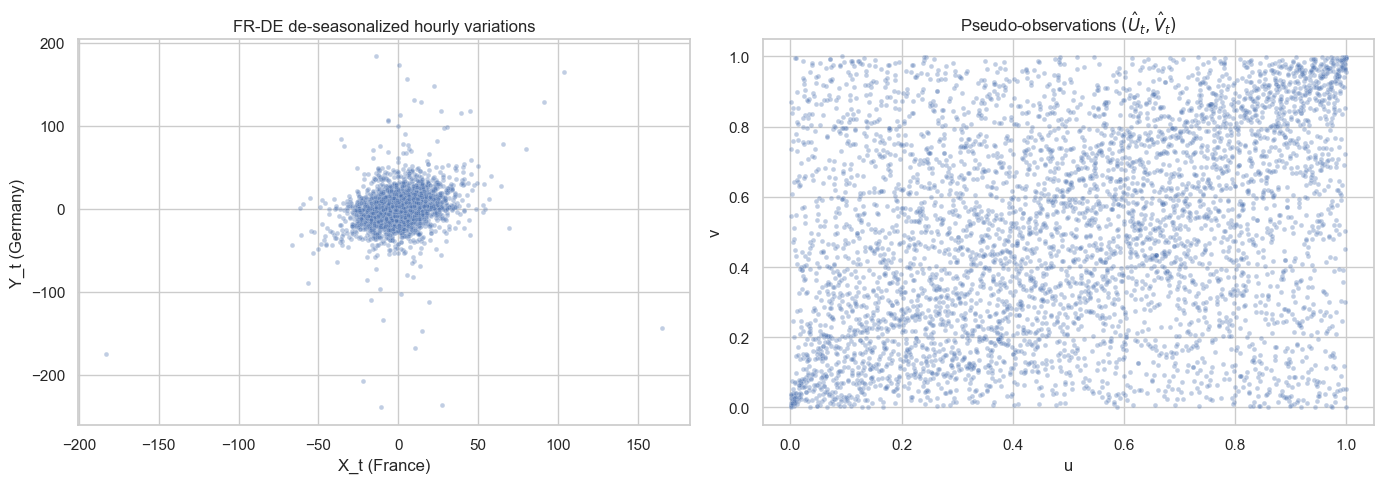
\includegraphics[width=0.96\textwidth]{figures/copula_scatter.png}
    \caption{Left: scatter plot of de-seasonalized hourly price variations in France and Germany. Right: pseudo-observations \((\hat U_t, \hat V_t)\) used for copula estimation.}
    \label{fig:copula_scatter}
\end{figure}

\subsection{Rank-based dependence measures}

We begin with nonparametric rank-based indicators. On the full sample, the Kendall coefficient is estimated at
\[
\hat\tau = 0.2177,
\]
while the Spearman coefficient is
\[
\hat\rho = 0.3062.
\]

These values indicate a positive but moderate dependence between the two markets. The two price series are clearly linked, but not in a way that would suggest near-deterministic co-movement. This makes the copula approach relevant: there is enough dependence to be modeled, but enough flexibility left to distinguish between alternative dependence structures.

\subsection{Parametric copula families}

We estimate three parametric copula families that were studied in the course: the Gaussian copula, the Gumbel copula, and the Clayton copula. The Gaussian copula is a natural benchmark but does not exhibit tail dependence. By contrast, the Gumbel copula captures upper-tail dependence, whereas the Clayton copula captures lower-tail dependence. This distinction is especially relevant for electricity prices, where the economic interpretation of very high prices and very low or negative prices is quite different.

For each family, we consider two estimation strategies: inversion of Kendall's tau and maximum likelihood based on the pseudo-observations. We then compare the fitted models through their log-likelihood, AIC, BIC, and implied tail-dependence coefficients.

Table~\ref{tab:copula_full} reports the results on the full sample.

\begin{table}[H]
\centering
\caption{Copula estimation results on the full sample.}
\label{tab:copula_full}
\begin{tabular}{lcccccccc}
\toprule
Family & \(\hat\tau\) & \(\hat\rho\) & Param. (tau) & Param. (MLE) & \(\ell_{\text{tau}}\) & \(\ell_{\text{MLE}}\) & \(\lambda_l\) & \(\lambda_u\) \\
\midrule
Gaussian & 0.2177 & 0.3062 & 0.3353 & 0.3113 & 294.6647 & 297.0064 & 0.0000 & 0.0000 \\
Gumbel   & 0.2177 & 0.3062 & 1.2783 & 1.2773 & 392.1663 & 392.1692 & 0.0000 & 0.2794 \\
Clayton  & 0.2177 & 0.3062 & 0.5566 & 0.3938 & 215.6555 & 245.2915 & 0.1720 & 0.0000 \\
\bottomrule
\end{tabular}
\end{table}

The ranking is unambiguous on the full sample: the Gumbel copula clearly dominates the Gaussian and Clayton alternatives. It yields the highest log-likelihood and the best information criteria, which indicates that the dependence between the two markets is better described by an asymmetric structure with upper-tail dependence than by a symmetric Gaussian benchmark or a lower-tail-dependent Clayton copula.

This result is economically meaningful. It suggests that the strongest common dependence between the French and German markets does not occur primarily during jointly very low prices, but rather during jointly high price episodes. In other words, the two markets appear especially connected when upward stress affects both systems at the same time.

\subsection{Calm versus stressed regimes}

To go beyond the average dependence structure, we split the sample into a calm regime and a stressed regime, based on large spread or volatility conditions. The purpose is not only to determine which copula performs best overall, but also to understand whether the form of dependence changes across market regimes.

Table~\ref{tab:copula_regimes} summarizes the corresponding estimates.

\begin{table}[H]
\centering
\caption{Copula estimation results by regime.}
\label{tab:copula_regimes}
\begin{tabular}{llcccccc}
\toprule
Regime & Family & \(\hat\tau\) & \(\hat\rho\) & Param. (MLE) & \(\ell_{\text{MLE}}\) & \(\lambda_l\) & \(\lambda_u\) \\
\midrule
Calm     & Gaussian & 0.2231 & 0.3168 & 0.3659 & 237.2648 & 0.0000 & 0.0000 \\
Calm     & Gumbel   & 0.2231 & 0.3168 & 1.3341 & 299.8596 & 0.0000 & 0.3187 \\
Calm     & Clayton  & 0.2231 & 0.3168 & 0.5021 & 195.2759 & 0.2514 & 0.0000 \\
Stressed & Gaussian & 0.2073 & 0.2888 & 0.2364 & 75.9999  & 0.0000 & 0.0000 \\
Stressed & Gumbel   & 0.2073 & 0.2888 & 1.1926 & 107.9107 & 0.0000 & 0.2118 \\
Stressed & Clayton  & 0.2073 & 0.2888 & 0.2633 & 67.7384  & 0.0719 & 0.0000 \\
\bottomrule
\end{tabular}
\end{table}

Several points emerge from this comparison. First, the Gumbel copula remains the best-performing family in both regimes, which makes the main conclusion robust. Second, the overall rank dependence is slightly stronger in the calm regime than in the stressed regime, as seen from both Kendall's tau and Spearman's rho. Third, upper-tail dependence remains present in both regimes, but is estimated to be larger in the calm regime than in the stressed one.

At first sight, the last point may seem surprising. One might expect stronger upper-tail dependence precisely during stressed periods. However, our stress partition captures high-volatility or large-spread situations more broadly, which may include heterogeneous episodes in which the two markets do not always move to the same extreme at the same time. In that sense, the stressed regime may contain more dispersion and more local asymmetries, even though it remains more turbulent.

\subsection{Empirical copula diagnostics and tail concentration}

Figure~\ref{fig:copula_heatmap} shows the empirical copula heatmap, while Figure~\ref{fig:copula_contours} presents the fitted contours for the three parametric families. These figures are useful because they complement the likelihood-based comparison with a direct visual representation of the dependence structure.

\begin{figure}[H]
    \centering
    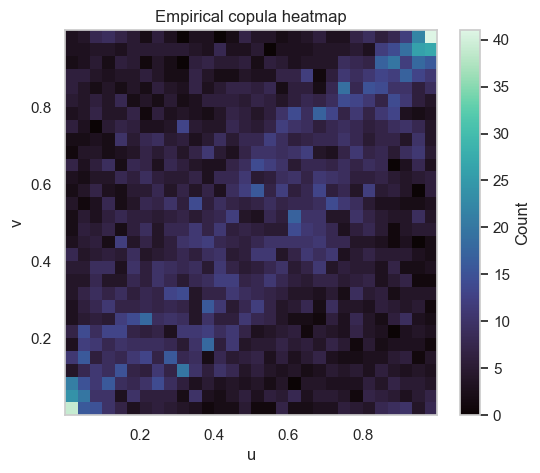
\includegraphics[width=0.58\textwidth]{figures/copula_heatmap.png}
    \caption{Empirical copula heatmap based on the pseudo-observations.}
    \label{fig:copula_heatmap}
\end{figure}

\begin{figure}[H]
    \centering
    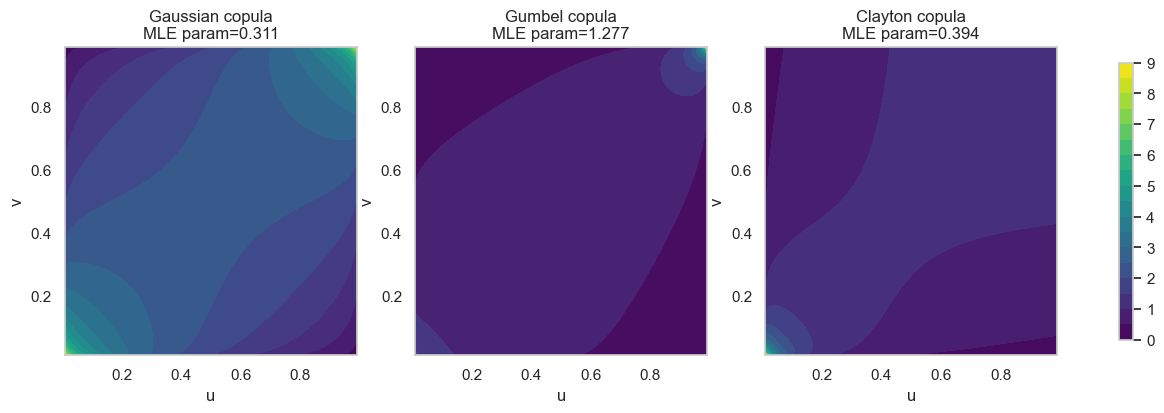
\includegraphics[width=\textwidth]{figures/copula_contour.png}
    \caption{Fitted copula contours for the Gaussian, Gumbel, and Clayton models.}
    \label{fig:copula_contours}
\end{figure}

We also examine empirical tail concentration functions in order to compare the lower and upper corners of the unit square. The lower-tail concentration decreases slowly and then appears to converge to zero for very small values of \(q\), which is not consistent with a very strong lower-tail dependence. By contrast, the upper-tail concentration is more structured: on the full sample it remains clearly positive, while in the stressed regime it becomes more irregular and even increases at very small values of \(q\). Although the smallest-\(q\) region must be interpreted cautiously because of limited sample size, this pattern is coherent with the dominance of the Gumbel family.

\begin{figure}[H]
    \centering
    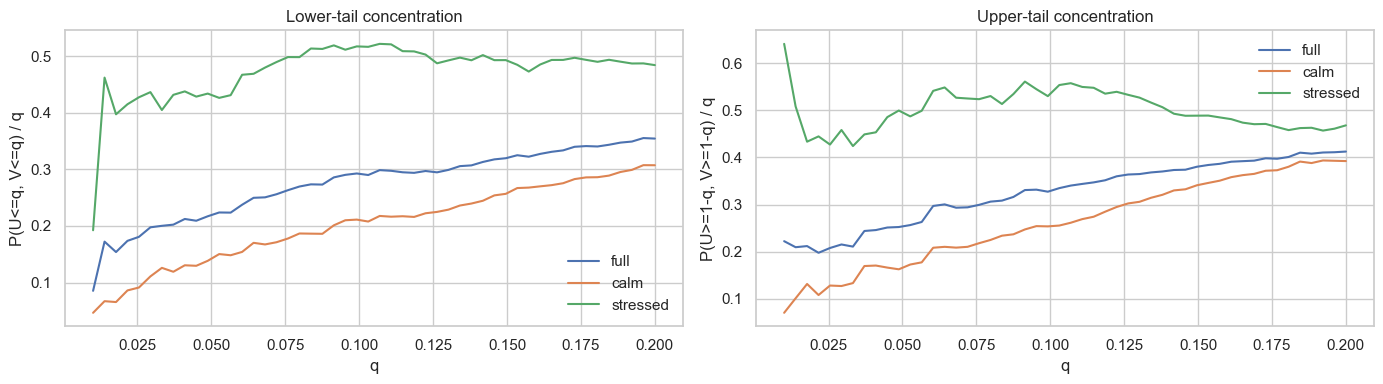
\includegraphics[width=\textwidth]{figures/copula_concentration.png}
    \caption{Empirical lower-tail and upper-tail concentration functions across regimes.}
    \label{fig:tail_concentration}
\end{figure}

\subsection{Interpretation}

Overall, the copula analysis shows that the dependence between French and German day-ahead prices cannot be reduced to average linear co-movement. The best-fitting copula is consistently the Gumbel copula, which points to an asymmetric dependence structure with upper-tail dependence. In economic terms, this means that the most informative joint behavior appears during common upward price stress, rather than during jointly very low or negative prices.

This conclusion complements the previous sections of the report. Once the marginal time-series dynamics have been accounted for, and once rare events have been identified through the extreme-value analysis, the copula framework reveals that dependence itself becomes more informative in the upper tail. This motivates the final step of our study: if extreme events occur jointly across markets, do they also cluster in time? This is the question addressed by the Hawkes-process analysis.

% ==========================================
% 6. HAWKES PROCESSES
% ==========================================
\section{Hawkes Processes for Extreme Event Clustering}
\label{sec:hawkes}
Copulas describe cross-market dependence, but they do not capture the temporal clustering of extreme events. In electricity markets, this temporal dimension is essential: once a market enters a stressed state, extreme prices often do not occur in isolation, but rather in bursts. For this reason, we model extreme events using Hawkes processes.

A Hawkes process is a self-exciting point process whose intensity depends on past events. In the multivariate setting, each component may also be excited by events occurring in the other component, which makes the framework particularly suitable for studying cross-market propagation. The process is stationary when the spectral radius of the branching matrix is strictly less than one.

\subsection{From hourly prices to event times}

Rather than modeling prices themselves as a point process, we transform the hourly time series into timestamped events. This is more natural in the Hawkes framework and better aligned with the objective of studying clustering in rare episodes.

We consider several event definitions, including negative prices, very high prices above the empirical 99\% quantile, large hourly jumps, and extreme spreads. In the final analysis, we focus on two economically meaningful cases: negative prices and very high prices. The negative-price case captures episodes of excess supply or severe market imbalance, while the high-price case captures upward stress episodes.

Table~\ref{tab:hawkes_event_counts} summarizes the frequency of the different event types.

\begin{table}[H]
\centering
\caption{Number and share of extreme events in France and Germany.}
\label{tab:hawkes_event_counts}
\begin{tabular}{lcccc}
\toprule
Event type & FR count & DE count & FR share & DE share \\
\midrule
Negative price      & 434 & 459 & 0.0741 & 0.0784 \\
High price 95\%     & 293 & 293 & 0.0500 & 0.0500 \\
Jump 95\%           & 293 & 293 & 0.0500 & 0.0500 \\
Spread extreme 95\% & 293 & 293 & 0.0500 & 0.0500 \\
High price 99\%     & 59  & 59  & 0.0101 & 0.0101 \\
\bottomrule
\end{tabular}
\end{table}

These frequencies justify the event-based approach. Negative prices are rare enough to be interpreted as stress events, but still numerous enough to support estimation. The same is true, more restrictively, for the upper 1\% price events.

\subsection{Univariate Hawkes analysis: negative prices}

We begin with univariate Hawkes processes estimated separately on the French and German negative-price events. We use an exponential kernel
\[
\phi(t) = \alpha e^{-\beta t}\mathbf{1}_{t>0},
\]
so that the branching ratio is given by \(\alpha/\beta\).

The observation window spans 6549 hours, with 434 negative-price events in France and 459 in Germany. Table~\ref{tab:hawkes_uni_negative} reports the corresponding estimates.

\begin{table}[H]
\centering
\caption{Univariate Hawkes estimates for negative-price events.}
\label{tab:hawkes_uni_negative}
\begin{tabular}{lccccccc}
\toprule
Country & \(\mu\) & \(\alpha\) & \(\beta\) & Branching ratio & \(\bar{\lambda}\) & Endogenous share & Log-likelihood \\
\midrule
France   & 0.0139 & 0.4935 & 0.6240 & 0.7909 & 0.0663 & 0.7909 & -1073.1962 \\
Germany  & 0.0148 & 0.5065 & 0.6415 & 0.7895 & 0.0701 & 0.7895 & -1119.8032 \\
\bottomrule
\end{tabular}
\end{table}

The baseline intensities are small in both countries, whereas the branching ratios are close to 0.79. This is a strong indication of self-excitation: once a negative-price event occurs, the probability of observing another similar event shortly afterward increases substantially. In both markets, roughly four-fifths of the total event activity is attributed to endogenous dynamics rather than to exogenous shocks.

This result confirms that negative prices are temporally clustered. They do not arrive as isolated points in time, but rather in bursts, which is exactly the kind of structure that a Hawkes process is designed to detect.

Figure~\ref{fig:hawkes_negative_timeline} presents the event raster plot over the full sample, while Figure~\ref{fig:hawkes_negative_intensity} shows the fitted univariate intensities.

\begin{figure}[H]
    \centering
    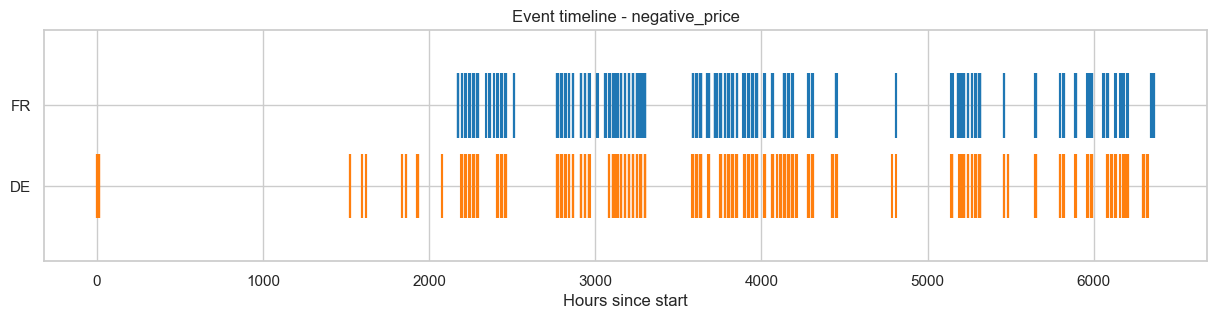
\includegraphics[width=0.8\textwidth]{figures/hawkes_negative_timeline.png}
    \caption{Timeline of negative-price events in France and Germany over the full sample.}
    \label{fig:hawkes_negative_timeline}
\end{figure}

\begin{figure}[H]
    \centering
    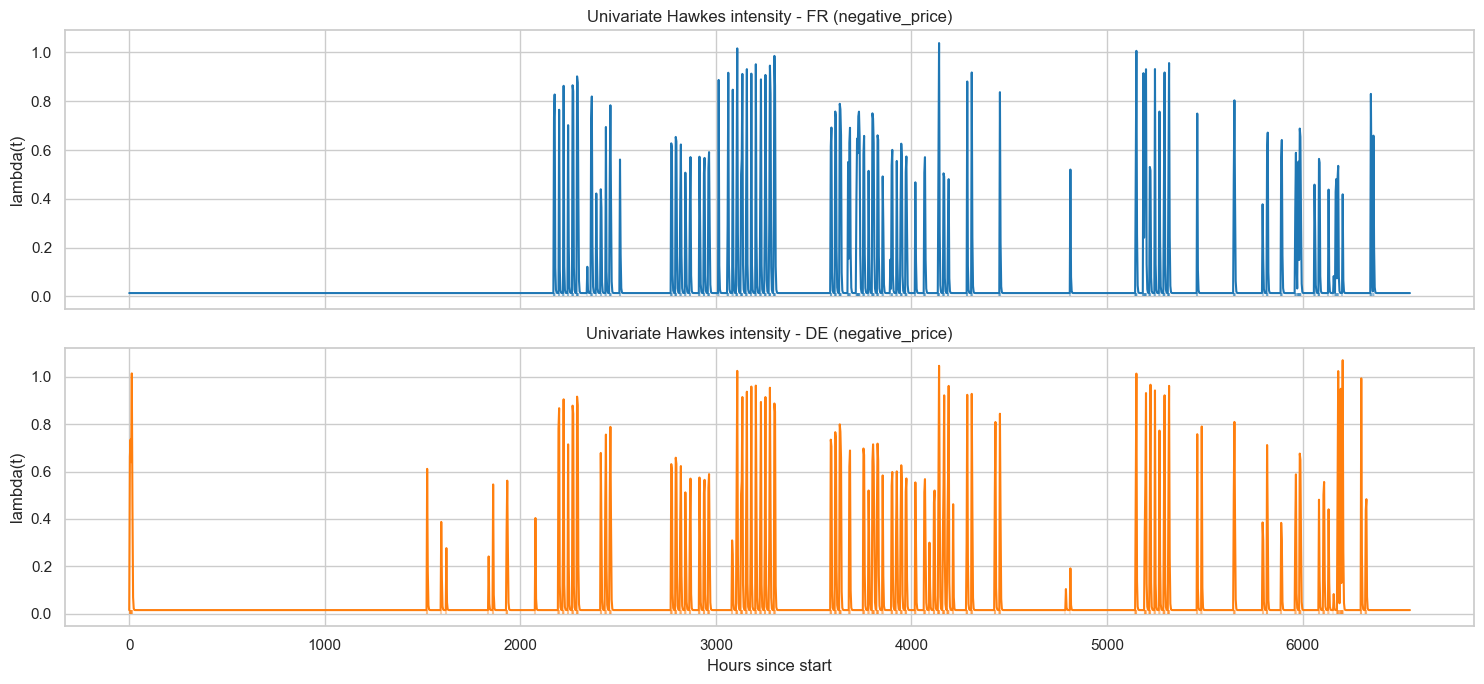
\includegraphics[width=\textwidth]{figures/hawkes_negative_intensity.png}
    \caption{Estimated univariate Hawkes intensities for negative-price events in France and Germany.}
    \label{fig:hawkes_negative_intensity}
\end{figure}

\subsection{Bivariate Hawkes analysis: negative prices}

We then estimate a bivariate Hawkes process in order to distinguish self-excitation from cross-excitation between the French and German markets. The fitted model yields the following branching matrix:
\[
G =
\begin{pmatrix}
0.6886 & 0.1321 \\
0.0308 & 0.7672
\end{pmatrix},
\]
with spectral radius
\[
\rho(G) = 0.8028 < 1.
\]

The stationarity condition is therefore satisfied. The model is stable, and the estimated long-run average intensities are \(\bar\lambda_{FR} \approx 0.0663\) and \(\bar\lambda_{DE} \approx 0.0701\).

Several features are noteworthy. First, both diagonal terms are large, which confirms strong self-excitation in each market. Second, cross-excitation is clearly asymmetric: the effect from Germany to France is larger than the reverse effect. More precisely, an extreme negative-price event in Germany appears to increase the short-term probability of a corresponding event in France more strongly than the opposite channel.

This asymmetry is economically plausible. It suggests that, for negative prices, the German market plays a stronger propagating role within the French-German pair. At the same time, the diagonal terms remain dominant, which means that local persistence is stronger than cross-border contagion.

Table~\ref{tab:hawkes_bi_negative} summarizes the bivariate estimates.

\begin{table}[H]
\centering
\caption{Bivariate Hawkes estimates for negative-price events.}
\label{tab:hawkes_bi_negative}
\begin{tabular}{lccc}
\toprule
Country & \(\mu\) & \(\bar{\lambda}\) & Endogenous share \\
\midrule
France  & 0.0114 & 0.0663 & 0.8283 \\
Germany & 0.0143 & 0.0701 & 0.7963 \\
\bottomrule
\end{tabular}
\end{table}

\begin{table}[H]
\centering
\caption{Estimated excitation matrix for negative-price events.}
\label{tab:hawkes_negative_matrix}
\begin{tabular}{lcc}
\toprule
Target / Source & FR source & DE source \\
\midrule
FR target & 0.6886 & 0.1321 \\
DE target & 0.0308 & 0.7672 \\
\bottomrule
\end{tabular}
\end{table}

Figure~\ref{fig:hawkes_negative_matrix} visualizes this excitation matrix, and Figure~\ref{fig:hawkes_negative_zoom} provides a zoom on the most tense week of the year.

\begin{figure}[H]
    \centering
    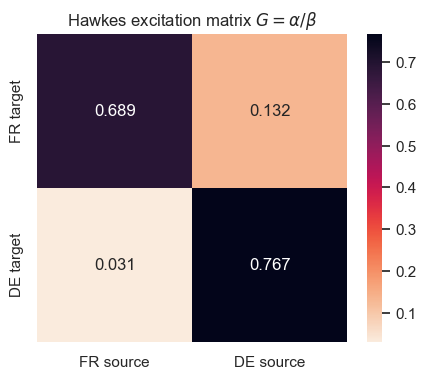
\includegraphics[width=0.45\textwidth]{figures/hawkes_negative_matrix.png}
    \caption{Estimated excitation matrix for the bivariate Hawkes model on negative-price events.}
    \label{fig:hawkes_negative_matrix}
\end{figure}

\begin{figure}[H]
    \centering
    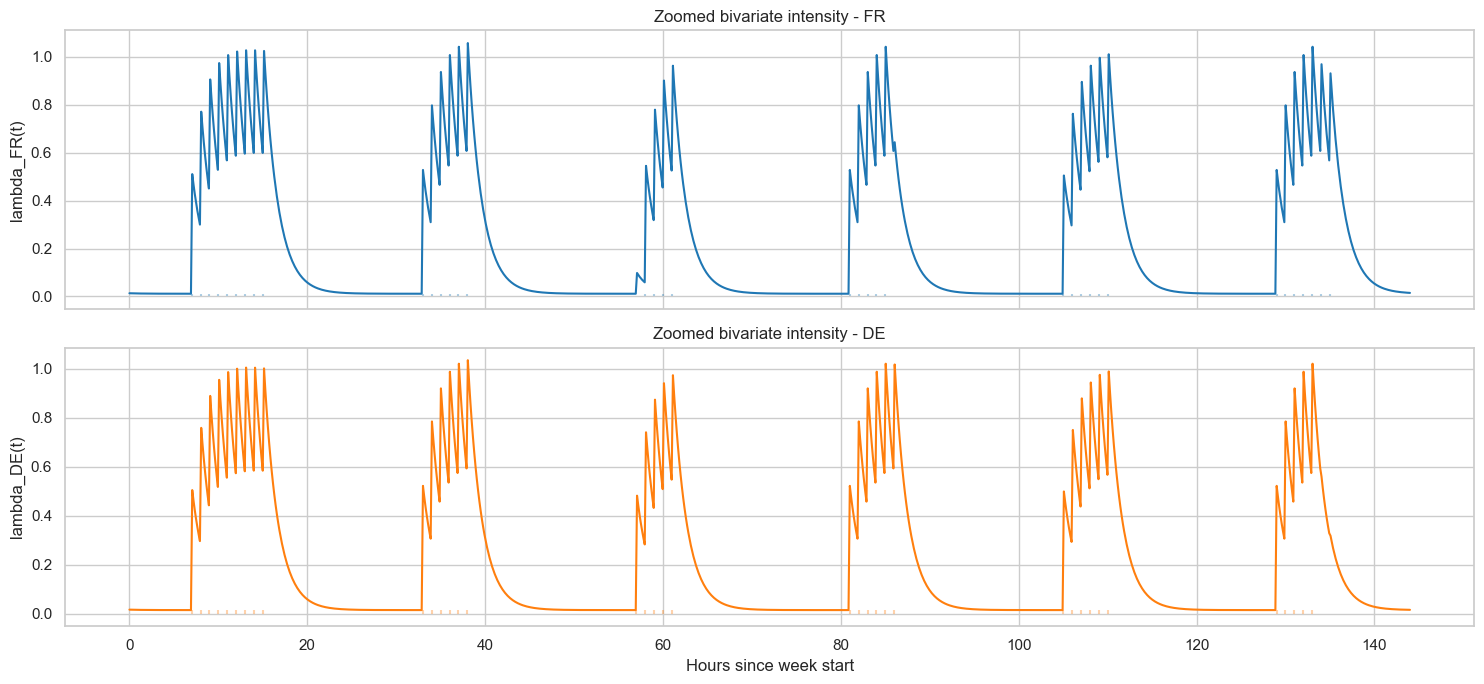
\includegraphics[width=0.8\textwidth]{figures/hawkes_negative_zoom.png}
    \caption{Zoom on a tense week for negative-price events and fitted bivariate intensities.}
    \label{fig:hawkes_negative_zoom}
\end{figure}

\subsection{Very high prices: upper 1\% events}

We perform the same analysis on very high prices, defined as observations above the empirical 99\% quantile. In this case, the observation window is again 6549 hours, but only 59 events are recorded in each country. These events are therefore much rarer than negative prices, which makes them especially relevant as indicators of severe upward market stress.

The univariate estimates are reported in Table~\ref{tab:hawkes_uni_high}. They again reveal self-excitation, with branching ratios of 0.8391 for France and 0.6663 for Germany.

\begin{table}[H]
\centering
\caption{Univariate Hawkes estimates for high-price 99\% events.}
\label{tab:hawkes_uni_high}
\begin{tabular}{lccccccc}
\toprule
Country & \(\mu\) & \(\alpha\) & \(\beta\) & Branching ratio & \(\bar{\lambda}\) & Endogenous share & Log-likelihood \\
\midrule
France   & 0.0014 & 0.1001 & 0.1193 & 0.8391 & 0.0090 & 0.8391 & -221.1900 \\
Germany  & 0.0031 & 0.1242 & 0.1864 & 0.6663 & 0.0093 & 0.6663 & -250.7652 \\
\bottomrule
\end{tabular}
\end{table}

The French series exhibits particularly strong self-excitation for upper-tail events. Once a very high price occurs in France, the fitted model indicates a high short-run probability of another high-price event shortly afterward. Germany also displays clustering, though less strongly.

The bivariate model leads to the branching matrix
\[
G =
\begin{pmatrix}
0.8271 & 0.0128 \\
0.1739 & 0.5234
\end{pmatrix},
\]
with spectral radius
\[
\rho(G) = 0.8343 < 1.
\]

Again, the stationarity condition is satisfied. The diagonal terms are large, especially for France, which confirms strong within-market clustering of upper-tail events. The cross-excitation terms are smaller than in the negative-price case and are also asymmetric, but now in the opposite direction: the effect from France to Germany is larger than the effect from Germany to France.

This difference between negative-price events and upper-tail events is particularly interesting. It suggests that the direction of cross-market propagation depends on the nature of the stress event. Negative-price episodes appear more strongly transmitted from Germany toward France, whereas very high price events appear more strongly transmitted from France toward Germany.

The corresponding summary tables are reported below.

\begin{table}[H]
\centering
\caption{Bivariate Hawkes estimates for high-price 99\% events.}
\label{tab:hawkes_bi_high}
\begin{tabular}{lccc}
\toprule
Country & \(\mu\) & \(\bar{\lambda}\) & Endogenous share \\
\midrule
France  & 0.0014 & 0.0090 & 0.8401 \\
Germany & 0.0028 & 0.0091 & 0.6957 \\
\bottomrule
\end{tabular}
\end{table}

\begin{table}[H]
\centering
\caption{Estimated excitation matrix for high-price 99\% events.}
\label{tab:hawkes_high_matrix}
\begin{tabular}{lcc}
\toprule
Target / Source & FR source & DE source \\
\midrule
FR target & 0.8271 & 0.0128 \\
DE target & 0.1739 & 0.5234 \\
\bottomrule
\end{tabular}
\end{table}

\subsection{Interpretation}

Taken together, the Hawkes analysis shows that extreme events are strongly clustered in time and exhibit measurable cross-excitation between the French and German markets. This cross-market propagation is asymmetric and depends on the event definition: negative-price episodes appear to spill over more strongly from Germany to France, whereas upper-tail events show the opposite pattern. In this sense, the Hawkes framework complements the copula analysis by adding a temporal dimension to joint extremes, showing that stress in the French-German day-ahead market is not only cross-sectional but also dynamically propagated over time.

% ==========================================
% 7. RESULTS AND DISCUSSION
% ==========================================
\section{Results and Discussion}
\label{sec:results}
The four methods used in this report provide complementary information on the same empirical question. The linear time-series analysis highlights the strong hourly and weekly structure of the market. The extreme-value analysis shows that rare and economically meaningful stress episodes remain an essential feature of the 2025 price distribution. The copula analysis reveals that dependence between France and Germany is not fully summarized by linear correlation and becomes especially informative in the tails. Finally, the Hawkes analysis shows that extreme events are temporally clustered and partially transmitted across markets.

Taken together, these findings suggest that market stress in the French-German electricity system has both a cross-sectional and a temporal dimension. Dependence matters because prices can become jointly extreme, and self-excitation matters because extreme events tend to arrive in bursts rather than in isolation. This joint perspective is one of the main contributions of the report.


% ==========================================
% 8. DATA AND CODE AVAILABILITY
% ==========================================
\section*{Data and Code Availability}

The data used in this report come from the ENTSO-E Transparency Platform, item \texttt{EnergyPrices\_12.1.D\_r3}, which provides day-ahead electricity prices by bidding zone and market time unit. The monthly files for 2025 can be accessed through the ENTSO-E file library at:

\url{https://transparency.entsoe.eu/fileLibrary/fileBrowserMode?appState=\%7B\%22path\%22\%3A\%22\%2FTP_export\%2FEnergyPrices_12.1.D_r3\%2F\%22\%7D}

The analysis was carried out in Python. In accordance with the course instructions, code is not included in the main report but was used to generate all tables and figures.

% ==========================================
% 9. CONCLUSION
% ==========================================
\section{Conclusion}
\label{sec:conclusion}

In this report, we studied French and German day-ahead electricity prices in 2025 through a unified statistical framework combining linear time-series methods, extreme-value analysis, copulas, and Hawkes processes. This organization made it possible to move progressively from marginal temporal structure, to tail behavior, to cross-sectional dependence, and finally to temporal clustering of extreme events.

Our results suggest that the French and German markets are linked by more than average co-movement. In particular, dependence becomes especially informative during stress episodes, where tail behavior and event clustering matter more than standard correlation. The copula analysis highlights asymmetric dependence patterns, while the Hawkes analysis shows that extreme events are not isolated but tend to propagate over time and, to some extent, across markets.

More broadly, the report illustrates the value of combining several tools from the course around a single coherent empirical question. Rather than presenting a juxtaposition of methods, we show that each technique answers a distinct part of the same problem: temporal dynamics, extreme risk, dependence structure, and self-excitation. This makes the French-German electricity market a natural and informative case study for statistical analysis in 2025.

% ==========================================
% 10. ACKNOWLEDGMENTS
% ==========================================
\section*{Acknowledgments}

We thank Mathieu Rosenbaum and the instructors of the course for their lectures and guidance. We also thank École Polytechnique for providing the academic environment in which this project was developed.

% ==========================================
% 11. AUTHOR CONTRIBUTIONS
% ==========================================
\section*{Author Contributions}

\textbf{Maxime Puech} conducted the linear time-series analysis, including the study of hourly and weekly seasonality, autocorrelation structure, and the preparation of transformed series used in later sections.

\textbf{Thaïs Roussel} carried out the extreme-value analysis, including the study of negative prices, large positive spikes, threshold exceedances, and the statistical characterization of rare events used to motivate the event definitions in the Hawkes section.

\textbf{Lucas Jung} conducted the copula-based dependence analysis and the Hawkes-process analysis, including the construction of pseudo-observations, the estimation and comparison of Gaussian, Gumbel, and Clayton copulas, and the modeling of temporal clustering and cross-excitation of extreme events.

All authors contributed to the interpretation of results, discussed the overall empirical strategy, and reviewed the final manuscript.

% ==========================================
% REFERENCES
% ==========================================
\bibliographystyle{plainnat}
\bibliography{references.bib}

\end{document}
